%\begin{titlepage}
\chapter*{}
\pagestyle{plain}

\begin{center}
\Huge{\textsc{Anexos}}
\end{center}

\addcontentsline{toc}{chapter}{Anexos}
%\end{titlepage}

\chapter*{}

\pagestyle{myheadings}
\markboth{ANEXOS}{ANEXO A}

\addcontentsline{toc}{section}{Anexo A: Código fuente}
\section*{Anexo A: Código fuente}
\subsection*{Clase para permitir movimiento autónomo al robot}
\lstinputlisting[language=c++, title={BaseCon.cpp}]{021-Anexo02-BaseCon.cpp}

\subsection*{Clase con la función de reconocer obstáculos en el plano}
\lstinputlisting[language=c++, title={Blobs.cpp}]{022-Anexo03-Blobs.cpp}
\lstinputlisting[language=c++, title={Blobs.hpp}]{023-Anexo04-Blobs.hpp}

\subsection*{Clase que representa al sensor MPU6050}
Esta clase se ocupa de inicializar al sensor y obtener los ángulos de inclinación del Robot.
\lstinputlisting[language=c++, title={Giro.cpp}]{024-Anexo05-Giro.cpp}

\subsection*{Utilitarios}
En este archivo se encuentran las funciones \texttt{calcular\_distancia()} y \texttt{calcular\_distancia\_horizontal()}, que calculan la distancia vertical y horizontal de un objeto detectado en el plano. También se encuentra la función \texttt{leerConfigFile()}, que sirve para leer archivos de configuración.

\lstinputlisting[language=c++, title={Utils.cpp}]{025-Anexo06-Utils.cpp}

\markboth{ANEXOS}{ANEXO B}
\addcontentsline{toc}{section}{Anexo B: Fotos del Robot}
\section*{Anexo B: Fotos del Robot}
%Robot con todos sus componentes instalados.

\begin{figure}
    \centering
    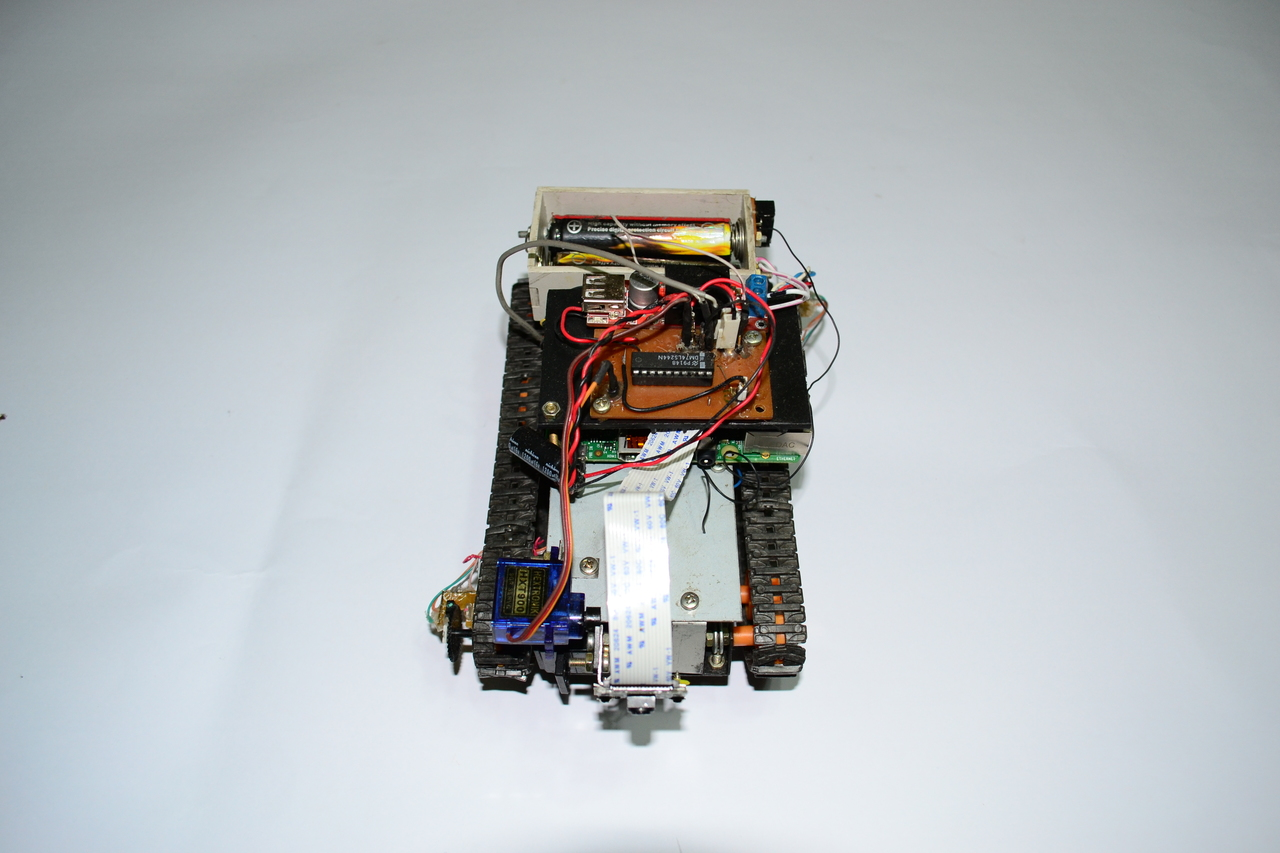
\includegraphics[width=0.8\textwidth]{r-DSC_0009.JPG}
    \caption{Vista frontal del robot. Se observa: el distribuidor de energía y regulador de voltaje al centro.}
\end{figure}

\newpage
\markboth{ANEXOS}{ANEXO C}
\addcontentsline{toc}{section}{Anexo C: Planilllas de seguimiento de sprint}
\section*{Anexo C: Planilllas de seguimiento de sprint}

\begin{table}
\centering
\begin{tabular}{|c|l|c|l|c|c|c|c|c|c|c|c|c|c|}
\hline
\multicolumn{4}{|r|}{} & 
V & L & M & X & J & V & L & M & X & J \\
\hline
\multicolumn{4}{|r|}{} & 
\rotatebox[origin=c]{90}{26-sep} & 
\rotatebox[origin=c]{90}{29-sep} & 
\rotatebox[origin=c]{90}{30-sep} & 
\rotatebox[origin=c]{90}{01-oct} & 
\rotatebox[origin=c]{90}{02-oct} & 
\rotatebox[origin=c]{90}{03-oct} & 
\rotatebox[origin=c]{90}{06-oct} & 
\rotatebox[origin=c]{90}{07-oct} & 
\rotatebox[origin=c]{90}{08-oct} & 
\rotatebox[origin=c]{90}{09-oct} \\
\hline
\multicolumn{4}{|r|}{\textbf{Tareas pendientes}} & 
9 & 8 & 8 & 8 & 8 & 5 & 4 & 2 & 2 & 2 \\
\hline
\multicolumn{4}{|r|}{\textbf{Horas pendientes}} & 
74 & 71 & 71 & 77 & 69 & 61 & 53 & 45 & 37 & 31 \\
\hline
\textbf{US} & \textbf{Tarea} & \textbf{Tipo} & \textbf{Estado} &
\multicolumn{10}{|c|}{\textbf{Esfuerzo}}\\
\hline
US1 &
T1 & Implementaci�n & Completada &
0 & 0 & 0 & 0 & 0 & 0 & 0 & 0 & 0 & 0 \\ 
\hline
US1 &
T2  & Investigaci�n & Completada &
0 & 0 & 0 & 0 & 0 & 0 & 0 & 0 & 0 & 0 \\ 
\hline
US1 &
T3 & Configuraci�n & Completada &
2 & 0 & 0 & 0 & 0 & 0 & 0 & 0 & 0 & 0 \\ 
\hline
US1 &
T4  & Investigaci�n & Completada &
0 & 0 & 0 & 0 & 0 & 0 & 0 & 0 & 0 & 0 \\ 
\hline
US1 &
T5  & Investigaci�n & Completada &
0 & 0 & 0 & 0 & 0 & 0 & 0 & 0 & 0 & 0 \\ 
\hline
US1 &
T6  & Implementaci�n & Completada &
5 & 4 & 4 & 10 & 2 & 0 & 0 & 0 & 0 & 0 \\
\hline
US1 &
T7  & Implementaci�n & Completada &
2 & 2 & 2 & 2 & 2 & 0 & 0 & 0 & 0 & 0 \\
\hline
US1 &
T8 & Pruebas & Completada &
2 & 2 & 2 & 2 & 2 & 0 & 0 & 0 & 0 & 0 \\
%--------
\hline
US2 &
T1  & Implementaci�n & Completada &
8 & 8 & 8 & 8 & 8 & 6 & 0 & 0 & 0 & 0 \\ 
\hline
US2 &
T2  & Implementaci�n & Completada &
8 & 8 & 8 & 8 & 8 & 8 & 6 & 0 & 0 & 0 \\ 
\hline
US2 &
T3  & Pruebas & Completada &
2 & 2 & 2 & 2 & 2 & 2 & 2 & 0 & 0 & 0 \\
%--------------------------------------------------------------------
\hline
US3 &
T1  & Implementaci�n & Pendiente &
20 & 20 & 20 & 20 & 20 & 20 & 20 & 20 & 12 & 6 \\
\hline
US3 &
T2  & Implementaci�n & Pendiente &
25 & 25 & 25 & 25 & 25 & 25 & 25 & 25 & 25 & 25 \\
\hline

\end{tabular}
\caption{Planilla de seguimiento del sprint A}
\label{table:planillaSPA}
\end{table}
%\end{landscape}
%\end{document}

